%************************************************
\chapter[\texttt{pystorms}]{A simulation sandbox for the development and evaluation of stormwater control algorithms}\label{ch:pystorms}
%************************************************

\vspace{1cm}

\section{Introduction}
\graffito{This chapter is developed in collaboration with \textbf{Sara P. Rimer} (Argonne National Laboratory) and \textbf{Sara C. Troutman} (University of Michigan).}


The advent of smart cities is poised to transform the management of our built environment \citep{Chourabi2012, Harrison2011}. Specific to stormwater, a new generation of smart and connected stormwater systems promises to reduce flooding and improve water quality management by autonomously sensing watershed parameters and subsequently controlling corresponding hydraulic components across complete watersheds, both \emph{adaptively} and \emph{in real-time}. These smart systems will provide an alternative to costly concrete-and-steel construction by squeezing even more performance out of existing stormwater and sewer infrastructure, and reimagining the design and operation of new infrastructure. While the idea of controlling distributed stormwater systems in real-time dates back to the 1970s \citep{Trotta1977}, the concept has only recently gained widespread traction in large part due to the affordability of internet-connected sensors, the increased capacity of data services, and the broader acceptance and popularity of other autonomous systems (e.g. self-driving cars and robots). Relative to other fields of autonomy, however, smart water systems are still early in their stage of adoption. Thus, developing and implementing smart water systems presents an exciting opportunity for researchers and practitioners alike to propose new visions, standards, and technologies.

 \
 
The intelligence of smart stormwater systems broadly refers to the acquisition (i.e. \dquote{sensing}) and processing of data into decisions and actions (i.e. \dquote{control strategies}) that are then used to guide the operation of gates, valves, pumps, and other actuators within a water system. Ultimately, the logic embedded via these control rules determines how water is moved around the collection system to meet specific performance objectives or reduce adverse outcomes (e.g. flooding, overflows, and/or water quality impairments). As such, the emerging field of smart stormwater systems stands to benefit greatly from researchers and stakeholders who can bring to bear new control strategies and techniques.

\

However, due to the complex, bureaucratic nature of watershed management, it can be impenetrable for new groups working in this field to obtain the necessary details of how real-world stormwater systems operate, as those details are unlikely to be opened up to just anyone who wants to try out new ideas of controlling them. To that end, computational toolchains exist for simulating stormwater systems and then evaluating various control rules implemented by them. Yet, developing these simulations and adapting them to specific control strategies often requires a significant amount of effort and expertise.  Furthermore, while a number of promising control algorithms have been proposed, they have all been evaluated on highly specific examples and simulators, making it difficult to establish cross-comparisons of their performance. In an effort to address these limitations, the contribution of this chapter is \pystormsNOSPACE, an open-source Python package comprised of:
%
\begin{enumerate}
\item A collection of real world-inspired smart stormwater control scenarios that facilitate the quantitative evaluation of control strategies, coupled with
\item A programming interface and a stormwater simulator to provide a stand alone package for developing stormwater control strategies.
\end{enumerate}
%
Our aspiration is for \pystorms to emerge as a community-driven resource that fosters accessibility and collaboration amongst smart stormwater control's field of researchers and practitioners, both novices and experts alike. 
%
%
%
%
%
%
%
%
%
%
%
%
%
%
%
% -------------------------------------------------------------------------------------------------------------------- %
\section{Background}
\label{sec:background}
% -------------------------------------------------------------------------------------------------------------------- %
%
%
%
\begin{figure*}
    \centering
    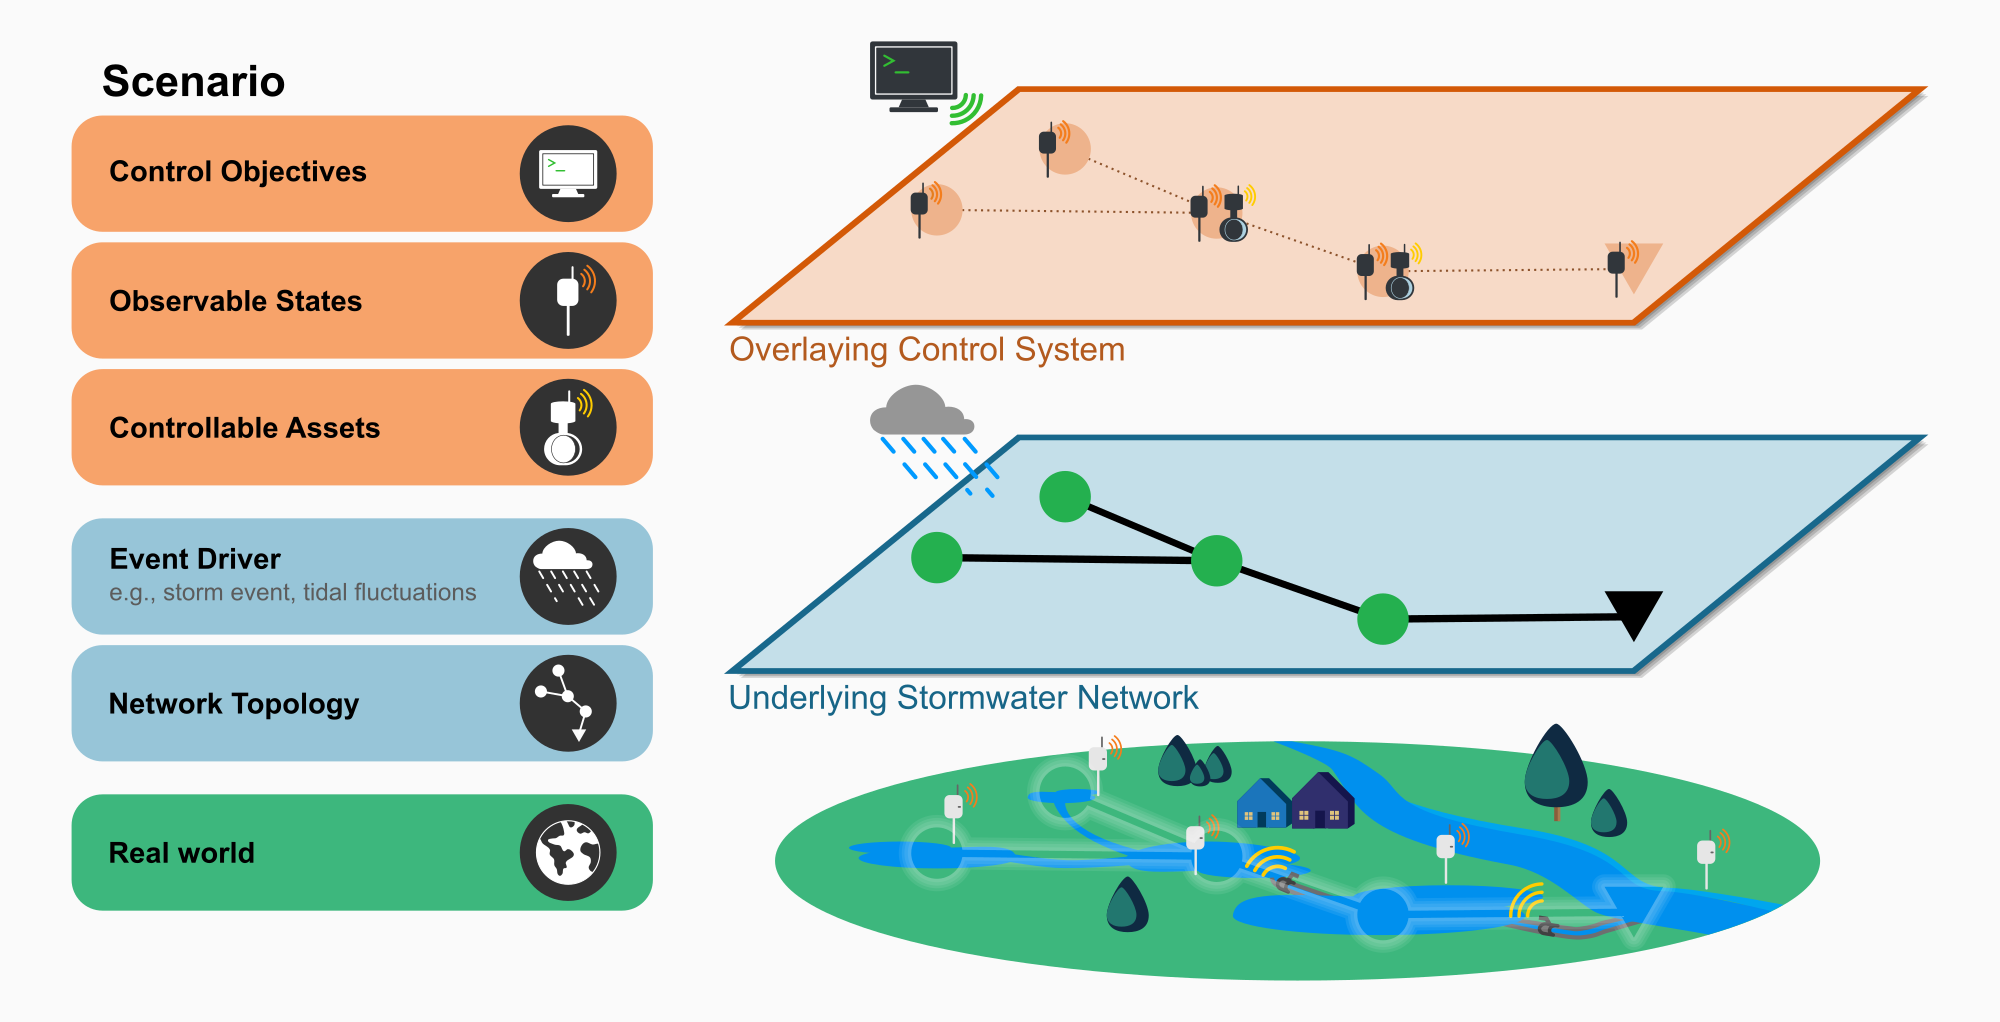
\includegraphics[width=\linewidth]{gfx/Chapter-5/pystormsLayersSketch.png}
    \caption{\pystorms abstracts the control of stormwater systems as scenarios, which are characterized by a computational representation of a stormwater network, a corresponding event driver, set of observable states, and controllable assets that can be leveraged to manipulate the behavior of a stormwater network in real-time to achieve control objectives. This is coupled with a streamlined programming interface and a stormwater simulator to provide the users with a standalone package for the development and evaluation of control algorithms.}
    \label{fig:scenarioComponents}
\end{figure*}
%
%
%
\subsection{Control of Stormwater Systems}
\label{subsec:controlofstormwatersystems}
%
%
%
A stormwater control problem can be defined as the development of an infrastructural strategy to manipulate the behavior of stormwater in order to achieve a desired response.
Traditionally, stormwater control has relied on \emph{passive} solutions, in which control strategies are large-scale, construction-heavy, and often financially-burdensome.
However, the emergence of microcontrollers, wireless communication technologies, and low-cost sensors has allowed for small-scale, modular, and automated control components (e.g. hydraulic valve operated by cellularly-connected actuator) to be installed at strategic locations throughout a stormwater network for \emph{active} control, with decisions that can be automated, adjusted remotely, and made in real-time.
Consequently, stormwater infrastructure can now be instantly redesigned to respond to its dynamic environment.

\

Although implemented smart stormwater control engineering solutions were documented at least a decade earlier, research-oriented discussion of these implementations did not occur until 1989 \citep{Schilling1989}.
Furthermore, while implementation of smart stormwater control began at the end of the 20th-century, the 21st-century has seen far more extensive systematic successes, as seen beginning with the foundational reviews of \citet{Schutze2004RealToday} and \citet{Vanrolleghem2005}.
Some notable adaptive real-time stormwater control implementations that have been installed hand-in-hand with extensive research dissemination include \citet{Ocampo-Martinez2010, Gaborit2013ImprovingForecasts, vezzaro2014,Gaborit2016, Mullapudi_Wong_Kerkez_2017, Montestruque2018, sadler2019}.
These references we specifically emphasize as to us they represent diverse and well-documented implementations of smart stormwater control from single control assets to watershed-scale implementations.
For more comprehensive reviews of stormwater control implementations, we direct the reader to some recently published survey articles on the topic \citep{Yuan2019, lund2018, shishegar2018optimization, VanDaal2017, Ocampo-Martinez_2015}. 
%
%
%
\subsubsection{Simulating Stormwater Systems}
\label{subsec:simulatingstormwatersystems}
%
%
%
Due to the variability of storm events and the safety concerns of experimental uncertainty, it is infeasible to test various control strategies on \emph{actual} stormwater networks. Thus, a more practical method to test the outcomes of different control decisions is to use a computational simulation of a stormwater network that is able to give us a \dquote{good enough} estimate of what the actual in-situ physical results might be. Often, these simulations can be carried out using computational stormwater models that have already been developed to inform the design and operation of the stormwater system being studied.

\

As a stormwater system is designed to route rainfall and other runoff to a wastewater treatment plant and/or discharge to a receiving body of water, the computational components of stormwater models primarily include a (i) runoff module and (ii) a routing module, and are driven by (iii) precipitation events (e.g. rain, snow). The runoff module converts precipitation into overland runoff; the overland runoff then undergoes hydrological processes (e.g. infiltration, evaporation) and is hydraulically transported to the stormwater collection system, which is carried out computationally via the routing module.

\

Over the years, several different software applications have been developed for modeling and simulating stormwater networks. The different software applications all function in a similar manner in which they computationally estimate the dynamics of stormwater as it moves through predefined temporal and spatial bounds to varying degrees of mathematical accuracy and fidelity to the underlying hydraulic and hydrological governing processes. The US-EPA's Stormwater Management Model (SWMM) \citep{Rossman2015a}, MIKE URBAN+ from the MIKE Powered by DHI software suite\footnote{\href{https://www.mikepoweredbydhi.com/products/mike-urban-plus}{mikepoweredbydhi.com}}, and the Model for Urban Stormwater Improvement Conceptualisation (MUSIC) by eWater\footnote{\href{https://ewater.org.au/products/music/}{ewater.org.au}} are a few examples of widely-used stormwater software applications. Furthermore, in addition to modeling runoff and its routing, some of these software applications have also been developed with the capabilities of modeling urban flooding (e.g. MIKE FLOOD) as well as the generation and transport of pollutants (e.g. SWMM). The computational details underlying the models produced by these software applications are not the purpose of this chapter, and instead for clarity and further detail, the reader is directed to \citet{Rossman2015b}, \citet{Rossman2017}, and \citet{Rossman2016}. Additionally, we provide further detail about the hydraulic simulator we utilize in Section \ref{subsec:architecture}.
%
%
%
\subsubsection{Implementing Control}
\label{subsec:implementingcontrol}
%
%
%
For those unfamiliar with control theory and control systems engineering, the field can be evasive. Here, we aim to maintain the idea of control in its broadest but most straightforward meaning: after receiving some sort of \emph{cue} (for our systems, this cue may be readings from sensors), an \emph{action} is taken on the system to alter it for a desired outcome (an action for stormwater systems may be as simple as the opening and closing of a valve). When we implement \emph{control}, we are making decisions and taking actions that try to optimize our system in order to meet some specified objective. Thus, a stormwater control strategy can be simplified as the method of developing rules that determine actions to be implemented by the stormwater system. The computational process of implementing this method to find these actions is what we define as the \emph{stormwater control algorithm}.

\

It is easy to imagine how finding the \dquote{best} actions to implement is a complex undertaking. Suppose a stormwater system with only one valve was installed, and that valve could be either completely opened or closed every hour. Deciding on a pattern for the complete opening and closing of the valve --- even over the period of a few days --- in order to meet some sort of objective is actually quite difficult, with no guarantee of a singularly \dquote{correct} solution. Now, imagine if the action could be to open the valve as a percentage between 0--100\% --- the combination of actions that can be implemented becomes even more endless. From an initial perspective, this process of finding the \dquote{best} and \dquote{correct} solution from what is an inexhaustible set of possibilities might seem futile. However, for stormwater applications, finding such an absolute \dquote{best} solution is usually not necessary, and most likely does not even exist. Instead, a solution that provides a \dquote{better} outcome than the current one is often sufficient and can still drastically benefit the system. Additionally, such better solutions are actually dependent on how a system's underlying needs are even defined. That is, \emph{how we define the objective determines what is considered optimal}. Thus, research on stormwater control focuses on both (i) the formulation of control objectives and (ii) analyzing and differentiating the myriad potential solutions based on said formulations. While the former research is essential in this field, it is not the focus of this chapter. Rather, our initiative here concentrates on the latter: via the presented simulation sandbox \pystormsNOSPACE, we aim to develop a systematic means for analyzing and differentiating control solutions for stormwater systems with pre-defined objectives.

\

Thus far, we have discussed \dquote{smart stormwater control} in its broadest sense, which encompasses all layers that a smart stormwater control system would entail --- from the sensors chosen, the communication protocol implemented for those sensors, the data management of what is sensed, the wireless actuators controlling a control asset, even to the human operators who may interact or intervene physically with the system. However, from here on out, we focus our discussion of smart stormwater control strategies strictly on \emph{the computational algorithm that is used to determine the discrete actions to be taken by the system's control assets based on information known regarding the system's past, current, and/or future state}. This algorithm can allow for the control strategy to be implemented and adjusted over any number of given time periods, and can be coordinated amongst any number of control assets within the system. By focusing strictly on the computational algorithm, we are able to isolate one component of smart stormwater systems that can allow for \emph{quantitative} cross-comparisons of strategies used across a multitude of stormwater systems. Additionally, the focus on the computational algorithm also centers the component of a smart stormwater system that can specifically benefit from experts outside the discipline of water resources engineering.
%
%
%
\subsection{The Need for a Simulation Sandbox}
\label{subsec:overviewofthesimulationsandbox}
%
%
%
Even though smart stormwater control has been successfully implemented for decades, there still does not exist a standard to systematically evaluate the performance of different control strategies across diverse stormwater networks and contexts. Consequently, this inability to systematically evaluate smart stormwater control directly impedes our field's ability to bring new and necessary expertise to solve some of our most essential and complex problems. 

\

As demonstrated by the smart stormwater control survey papers referenced in Section \ref{subsec:controlofstormwatersystems}, this desire for direct and systematized comparisons of control strategies is not an isolated realization. While there have been previous efforts to introduce benchmarking stormwater networks for evaluating control strategies \citep{Schutze2017, Borsanyi2008}, we identify the need to make available a more extensive assortment of example stormwater networks to the broader research community. This assortment of networks must be both nonexclusive and nonrestrictive, and capture the complexity and diversity of features unique to stormwater.
Furthermore, we recognize that there is a need for an unambiguous programming interface that explicates the computational backend and aids researchers to easily utilize the example networks for prototyping stormwater control solutions. 

\

We developed \pystorms as a Python-based \emph{simulation sandbox} to accelerate a researcher's ability to computationally simulate and evaluate stormwater control strategies. \pystorms provides a collection of diverse stormwater control scenarios, which are drawn from real-world urban watersheds to encompass diverse features appertaining to stormwater systems. These scenarios are coupled with a stormwater simulator and streamlined programming interface, which together provide researchers with a standalone package that focuses its usage on stormwater control algorithm development and testing. Our intention is that \pystorms reduces the programming learning curve that can be a barrier to those aspiring to learn stormwater control, and also curates an open repository of smart stormwater control examples which foster the development and evaluation of any number of new control strategies applied to them. In the following section, we present a detailed overview of the design and architecture of \pystormsNOSPACE, and how it facilitates the systematic evaluation of stormwater control strategies. 
%
%
%
\begin{table*}[ht]
\small
\caption{Terminology defined for the \pystorms package and to delineate stormwater scenarios.}\label{tab:terminology}
\begin{tabular}{l p{3.5in}}
\toprule
\textbf{Network Topology} & We distinguish a \emph{network} to be the physical system of conduits (e.g.\ pipes, culverts), storage elements (e.g.\ retention and detention basins), and any other subcatchment infrastructure (e.g.\ green infrastructure, wetlands) that collect, convey, and/or treat stormwater runoff. \\\midrule
\textbf{Event Driver} & Any inputs or ``disturbances'' to the network that govern the generation and flow of runoff are defined as event drivers.
Most often, an event driver is the precipitation generating runoff in the watershed.
It can also include wastewater flows, tidal fluctuations of connected water bodies, or any other such phenomenon that influence the flow of runoff in the network. \\\midrule
\textbf{Controllable Assets} & Any elements (e.g.\ basins, wetlands, CSO pump stations) that are equipped with valves, pumps, or any other flow control infrastructure that can be actuated to manipulate stormwater flow. \\\midrule
\textbf{Observable States} & The collection of states in the network (e.g.\ water levels, flows, pollutants) that can be accessed by the users during a simulation. \\\midrule
\textbf{Control Objectives} & The overall goal or set of goals (e.g.\ preventing flooding, improving water quality, reducing erosion) of manipulating the behavior of a stormwater network using controllable assets during a simulation.
The ability of a controller to achieve a particular objective is quantified using a performance metric. \\
\bottomrule
\end{tabular}
\end{table*}
%
%
%
%
%
%
%
%
%
%
%
%
%
%
%
% -------------------------------------------------------------------------------------------------------------------- %
\section{\pystorms}\label{sec:pystorms}
% -------------------------------------------------------------------------------------------------------------------- %
%
%
%
Developed in Python, \pystorms is supported on all major operating systems (OSX, Windows, and Linux) and can be installed using \texttt{pip}\footnote{\href{https://pypi.org/project/pystorms/}{pypi.org/project/pystorms}}.
\pystorms is distributed under the GNU General Public GPLv3 license\footnote{\href{https://www.gnu.org/licenses/gpl-3.0.html}{gnu.org/licenses/gpl-3.0.html}}, which ensures that this package and its derivatives remain open-source and can be used free of cost. Additionally, source code for the package is available on Github\footnote{\href{https://github.com/kLabUM/pystorms}{github.com/kLabUM/pystorms}}, alongside comprehensive documentation and tutorials to utilize and contribute to its broader development\footnote{\href{http://open-storm.org/pystorms}{open-storm.org/pystorms}}. 
%
%
%
\subsection{Scenarios}\label{subsec:scenarios}
%
%
%
\begin{table*}[ht]
\small
\caption{\pystorms includes a curated collection of real world-inspired stormwater scenarios for developing and quantitatively evaluating the performance of stormwater control algorithms.}\label{tab:scenarios}
\begin{tabular}{p{0.5in}p{1.75in}p{1.75in}}
\toprule
\textbf{Scenario} & \textbf{Network} & \textbf{Control Objectives} \\\midrule
\scenario{theta} & $2 \unit{km^2}$ idealized separated stormwater network & Maintain the flows at the outlet below a threshold and avoid flooding (2 storage basin outlets) \\\midrule
\scenario{alpha} & $0.12 \unit{km^2}$ residential combined sewer network & Minimize total combined sewer overflow volume (5 weirs at interceptor connections) \\\midrule
\scenario{beta} & $1.3 \unit{km^2}$ separated stormwater network with a tidally-influenced receiving river & Minimize flooding (1 detention pond outlet, 1 storage basin outlet, 1 pump) \\\midrule
\scenario{gamma} & $4 \unit{km^2}$ highly urban separated stormwater network & Maintain channel flows below threshold and avoid flooding (11 detention pond outlets) \\\midrule
\scenario{delta} & $1.7 \unit{km^2}$ combined sewer network in which the stormwater ponds also serve as waterfront & Maintain water levels within upper and lower thresholds for water quality and aesthetic objectives (5 storage basin outlets) \\\midrule
\scenario{epsilon} & $67 \unit{km^2}$ highly urban combined sewer network & Maintain sewer network outlet TSS load below threshold and avoid flooding (11 in-line storage dams) \\ \midrule
\scenario{zeta} & $1.8 \unit{km^2}$ combined and separated sewer network (based on the Astlingen benchmarking network \citep{Schutze2017, Sun_2020}) & Maximize flow to downstream wastewater treatment plant and minimize total combined sewer overflow volume (4 storage basin outlets) \\
\bottomrule
\end{tabular}
\end{table*}
%
%
%
\pystorms abstracts smart stormwater systems as \emph{scenarios}. Each scenario is described by (i) \emph{an underlying stormwater network}--which includes the network's topology (e.g.\ a sewer system draining into a water body) and its event driver (e.g.\ storm event)--and its \emph{overlaying control system}, which includes a set of observable states (e.g.\ water levels), controllable assets (e.g.\ basins with controllable valves at outlet), and a specific control objective (e.g.\ preventing flooding). The specific terminology for a scenario in \pystorms is described in further detail in Table~\ref{tab:terminology}, and the corresponding delineation between (i) and (ii) is illustrated in Fig.~\ref{fig:scenarioComponents}. 

\

By abstracting our stormwater systems as scenarios, we are able to create new scenarios with relative ease by interchanging different scenario components. For example, let us assume we have evaluated a control algorithm when applied to an individual scenario. We can now broaden our inquiry and test the algorithm's \emph{scalability} by interchanging components of our scenario's overlaying control system (e.g. sequentially increase its number of controllable assets), and evaluating the algorithm on this newly derived set of scenarios. Similarly, we can quantify the \emph{generalizability} of a control algorithm as it is applied to a specific control objective (e.g.\ maintaining water level set points) by systematically altering the underlying stormwater network (e.g. cycle through a set of design storms as the event driver) while retaining the overall control system. We can then calculate a performance metric of the algorithm when applied across this new subsequent set of scenarios. Thus, not only can can now evaluate a control algorithm applied to an individual stormwater scenario, but we can also evaluate it more universally when applied across a spectrum of these interchanged scenarios. 

\

\pystorms provides an collection of seven scenarios, drawn from real-world smart stormwater systems across North America and Europe and named as a letter from the Greek alphabet. The collection of scenarios span a multitude of stormwater systems that address a diverse set of urban watershed needs with various smart control objectives. The subcatchment areas range from $0.12 - 67 \unit{km^2}$ in size, and include both combined and separated stormwater arrangements. A brief summary of the collection's scenarios are presented in Table~\ref{tab:scenarios}.

\

While our aim is for this collection of scenarios to be representative of a myriad of smart stormwater control, we recognize that it is certainly not exhaustive. As such, we aspire to grow the \pystorms repository of stormwater scenarios through community-driven contributions of new scenarios. Accordingly, we provide extensive documentation \footnote{\href{https://www.pystorms.org/build/html/index.html}{open-storm.org/pystorms/docs/build-scenarios}} for users to contribute their own scenarios, or modify the existing ones. 

\

To demonstrate what is a scenario in the context of \pystormsNOSPACE, we present here Scenario \scenario{theta}, an idealized stormwater network that can be used for rapid prototyping of control strategies. Scenario \scenario{theta}'s \emph{network topology} can be described as two $1000 \unit{m^3}$ storage basins connected in parallel and draining through a shared outlet into a downstream water body. The \emph{event driver} is a synthetic rain event lasting $9 \unit{hr}$ with a peak intensity of $3.2 \unit{in}$. We stipulate the \emph{observable states} to be the water levels at the two basins at each $15 \unit{min}$ time-step of the simulation, and the \emph{controllable assets} are outlet valves of both storage basins adjustable at each time-step between $0-100\unit{\%}$ open. The \emph{control objective} is to maintain the outflow into the downstream water body below a specified threshold of $0.5 \unit{m^3s^{-1}}$, while simultaneously preventing flooding at the basins. The ability of a control strategy to meet \scenario{theta}'s control objective is quantified using a pre-defined performance metric that computes a penalty for violating the control objective at each time-step, and sums these penalties across the whole simulation. We provide the specific details on this performance metric (eq.~\ref{eq:perf-obj}) in Section~\ref{sec:evaluatingcontrolstrategies} where we evaluate the performance of two different example control strategies applied to \scenario{theta}.
%
%
%
\subsection{Programming Interface}
%
%
%
\begin{figure}[ht]
    \centering
	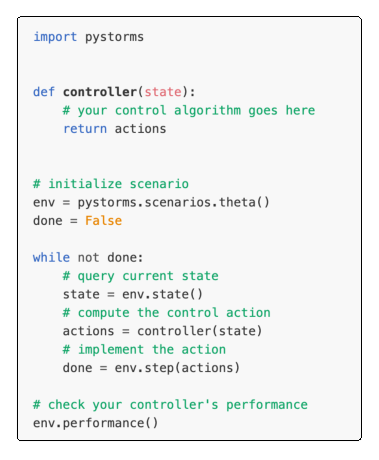
\includegraphics[width=0.9\linewidth]{gfx/Chapter-5/pystorms_code.eps}
	\caption{\pystorms provides a high-level abstraction for simulating control in stormwater networks for users to quantitatively evaluate the performance of control strategies with minimal overhead.}\label{fig:code}
\end{figure}
%
%
%
The \pystorms programming interface is inspired by the principles of control theory, where the control of a system is abstracted as an iterative process (also known as a control loop) in which a controller monitors the underlying state(s) of the system of interest, and makes calculated adjustments --- via control actions --- to the system for it to achieve a desired behavior. In the context of smart stormwater control, our system of interest is our stormwater network, and the states and control actions are represented by the set of observable states and the specific control asset configurations (e.g.\ valve positions and pump settings). Thus, we have discretized the simulation of stormwater control in \pystorms as the following series of steps:
%
\begin{enumerate}
	\item \label{query} \textbf{Query the set of observable states} for specified locations in the stormwater network at the current time-step; then potentially use these queried states to 
	\item \label{compute} \textbf{Compute control actions} to manipulate the system to achieve a desired behavior; and finally, 
	 \item \label{implement} \textbf{Implement the control actions} by adjusting the settings of the controllable assets that serve as inputs into the underlying system. 
\end{enumerate}

\

We initialize a \pystorms scenario by creating an instance of it using the statement:  \texttt{pystorms.scenarios.<scenario name>()}.
As seen in Fig.~\ref{fig:code}, \scenario{theta} is initialized with \texttt{pystorms.scenarios.theta()}.
The initialization then configures the stormwater simulator with the computational representations necessary to simulate the respective scenario, and returns it as a Python object. This Python object (\texttt{env} in Fig.~\ref{fig:code}) can be used to progress and/or pause the stormwater simulator, read and/or write parameters to the network, and utilize any additional \pystorms functionality. The current state of the underlying stormwater network in the scenario can be queried using the \texttt{<scenario object>.state()} call (\texttt{env.state()} in Fig.~\ref{fig:code}).
\texttt{<scenario object>.step(<actions>)} implements the control actions in the stormwater network, progresses the simulation forward a time-step, and returns the current status of simulation (\texttt{True} when the simulation has terminated and \texttt{False} otherwise). In Fig.~\ref{fig:code}, \texttt{done = env.step(actions)} implements \texttt{actions} in the stormwater network and progresses the simulation being handled by the \texttt{env} Python object, which in this case is the Scenario \scenario{theta}.
\texttt{done} is assigned \texttt{True} when the simulation has terminated, and \texttt{False} otherwise.


\

During the each time-step of the simulation, the ability for the implemented control actions to achieve the scenario's control objective are evaluated by computing the time-step's corresponding performance metric. This computed value is then stored for each time-step, and can be accessed at any time during the simulation using \texttt{<scenario object>.performance()} (\texttt{env.performance()} in Fig.~\ref{fig:code}). Additional parameters are logged throughout the simulation. While an initial set of these logged parameters is predefined, the user is able to customize this set for any additional parameters of interest. 

\

The series of steps for implementing a control loop into our stormwater simulation is seamlessly integrated throughout the \pystorms programming interface. Users carry out Step \ref{query} using \texttt{<scenario object>.\-state()}, and Step \ref{implement} using 
\texttt{<scenario object>.\-step(<actions>)}. Separated out to be defined by the user is the controller (Step \ref{compute}), which maps the observed states to control actions. While implementing the controller into \pystorms is ultimately left to the user, for our example presented here, we implement it as a Python function block (see Fig.~\ref{fig:code}).
%
%
%
\subsection{Architecture}
\label{subsec:architecture}
%
%
%
The \pystorms architecture follows the object oriented programming paradigm which relies on classes as its core building blocks. This style of software architecture was chosen to allow \pystorms to be modular such that users can customize it to meet their own specific requirements and/or workflows.  While the \pystorms programming interface is designed with the intent to be intuitive for all potential users, it particularly caters to those who may only have a rudimentary understanding of stormwater dynamics and/or basic familiarity with programming in Python. However, it can also be easily customized to meet the requirements of researchers who want to incorporate advanced functionality, such as custom water quality or rainfall-runoff modules (for details on how to utilize \pystorms modularity and customization, we again direct the reader to its online documentation). 

\

The \pystorms architecture is organized to accomplish two tasks: (1) the configuration of the scenario metadata, and (2) the simulation of the stormwater network. These two tasks are carried out using three core interacting modules: \texttt{environment}, \texttt{scenario}, and \texttt{config}. These three modules interface with each other to build and execute the various scenarios. Fig.~\ref{fig:arch} provides a schematic of this architecture. The first two modules handle the stormwater simulation, while the latter handles the computational representation of the stormwater networks and the metadata pertaining to the control problem (i.e.\ states, actions, and objectives). 
%
%
%
\begin{figure}[ht]
    \centering
	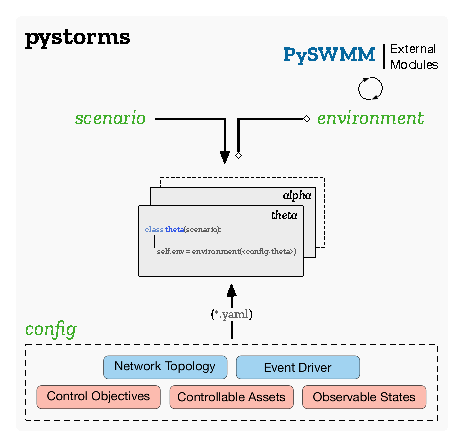
\includegraphics[width=\linewidth]{gfx/Chapter-5/pystorms_architectire_fin.eps}
	\caption{\pystorms is built with three interacting core modules: (i) \texttt{config} represents the metadata and computational representations of the stormwater network and event driver; (ii) \texttt{environment} acts as an interface for scenarios to interact with the stormwater simulators; and (iii) \texttt{scenario} provides a consistent structure for the scenarios in the package. A scenario object in \pystorms inherits (represented by arrows) from the base \texttt{scenario} class, and interfaces (represented by line) with the stormwater simulator though the \texttt{environment}. }\label{fig:arch}
\end{figure}
%
%
%
\subsubsection{Configuration}
%
%
%
The \texttt{config} module is used to manage the configuration in the \pystorms architecture. \texttt{config} contains a configuration file for each scenario, which delineates the stormwater network, its set of observable states and controllable assets, and the set of parameters that are used to compute its control objective's corresponding performance metric. The configuration files are written using YAML, a mark-up language commonly used for developing configuration files in software applications. With YAML, the parameters of interest defined in the configuration file are formatted as vertical lists rather than data structures. As a result, the configuration file becomes more human-readable, and creates a scalable and easy workflow for developing scenarios. 
%
%
%
\subsubsection{Simulation}
%
%
%
Scenarios in \pystorms are implemented as Python classes. To ensure consistent functionality across scenarios, each scenario is instantiated as its own independent class with an inherited structure from a base \texttt{scenario} module. The scenario classes interface their corresponding configuration files with the stormwater simulator and implement any of the functions specific to that scenario (e.g.\ functions used for computing performance metrics of corresponding control objectives).

\

The \texttt{environment} module is the interface between the stormwater simulator (e.g.\ EPA-SWMM) and the scenarios. This module is specifically included to ensure \pystorms is able to remain agnostic to whatever stormwater simulator is used. For instance, if a user wants to utilize a customized hydrologic solver for simulating stormwater, they can do so by modifying the \texttt{environment} module to call their solver when the scenarios query it, thus ensuring compatibility to a wide array of simulators with minimal overhead. 

\

\pystorms uses SWMM as its default stormwater simulator. SWMM, developed by the US-EPA, is an open-source stormwater simulation model that is extensively used for the design and analysis of stormwater systems across the world. SWMM is built with the C programming language, a low-level language that results in significant computational efficiency. However, the trade off for using C is SWMM's difficulty to be interfaced with the latest scientific libraries. As a result, there have been several efforts over the years to build wrappers for SWMM such that its functionality can be exploited via high-level programming languages, such as Python.  

\

PySWMM is a Python implemented package that not only provides a wrapper to communicate with SWMM, but also yields a high-level user interface for querying the various stormwater parameters. \pystorms --- by means of the \texttt{environment} module --- interfaces with SWMM using PySWMM, and as a result, all functionality included in PySWMM can also be accessed using \pystormsNOSPACE. Readers are directed to the documentation for additional details and examples to customize \pystorms to meet their requirements. 
%
%
%
\begin{figure}
    \centering
    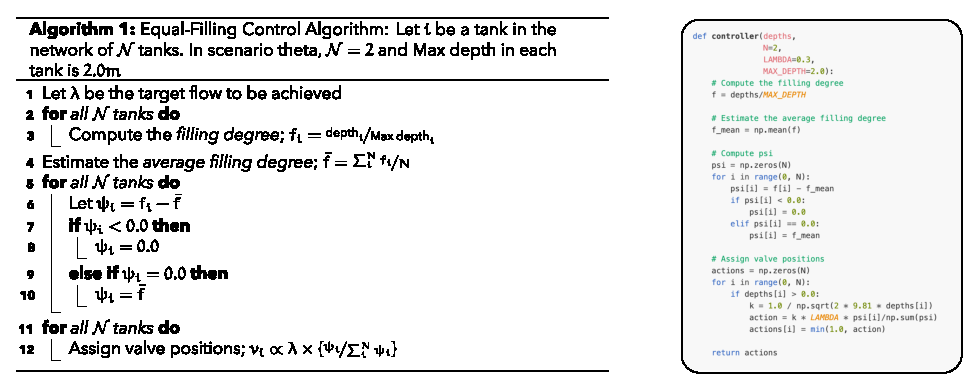
\includegraphics[width=\linewidth]{gfx/Chapter-5/algo.eps}
    \caption{Equal-filling controller maintains the flows at the outlet below a desired threshold by coordinating its actions such that it equally utilizes the storage in the controllable assets of the network.
    Algorithm 1 and the corresponding code snippet illustrate the algorithm and its Python implementation.}\label{fig:eqf}
\end{figure}
%
%
%
%
%
%
%
%
%
%
%
%
%
%
%
% -------------------------------------------------------------------------------------------------------------------- %
\section{Demo: Evaluating Control Strategies}
\label{sec:evaluatingcontrolstrategies}
% -------------------------------------------------------------------------------------------------------------------- %
%
%
%
Throughout this section, we demonstrate how \pystorms facilitates developing smart stormwater control strategies by evaluating the performance of two control algorithms applied to Scenario \scenario{theta}.

\

While there exist many control strategies that can be adopted to achieve \scenario{theta}'s control objective, to simplify our illustration of \pystormsNOSPACE, we implement two basic control strategies here. The algorithms used to implement the control strategies are described below and in Fig.~\ref{fig:eqf}. Both control strategies are simple reactive control strategies, in which the valve settings of \scenario{theta}'s two basin outlets are adjusted to either retain or release storage depending on the observed states compared some corresponding water level limits. 
%
%
%
\paragraph{Rule-based Control}
Our basic rule-based control strategy adjusts our basin outlets based on their respective water levels. Specifically, each basin's outlet setting is equal to its relative water level (i.e., the current water level of the basin divided by its maximum depth). Therefore, our control algorithm will set a full basin's outlet to 100\% open, and a basin that is half full will have its outlet set to 50\% open, etc. While this strategy provides a means to mitigate local flooding at each basin, it notably does not consider the other control objective for the network's outflow into the downstream water body to stay below a given threshold.
%
%
%
\paragraph{Equal-filling Degree Control}
The equal-filling degree is a control strategy often applied to stormwater networks with distributed stormwater storage assets, and has commonly been used as a starting point when comparing more than one control strategies \citep{Borsanyi2008, Campisano2000, Dirckz2011, Kroll2016, vezzaro2014}. For this strategy, we begin by defining a storage asset's ``filling degree'' --- which is typically the ratio a storage asset is full based on its volume or depth --- and compute it for each asset in the collection system. The algorithm seeks to ``balance'' these filling degrees across the system based on its average. The exact manner in which this balancing is carried out is not necessarily consistent in literature. Our method for this balancing is delineated in the algorithm in Fig.~\ref{fig:eqf}. If all assets have a filling degree equal to the average (i.e., all assets are equally filled), then each should release an equal fraction of the target outflow. Otherwise, the released flows across the assets should be differentiated such that, when an asset has a filling degree less than the average, it does not release any flow; but if an asset is greater than the average, it releases flows based on its deviation from the average. 

\

The implementation of the equal-filling degree algorithm using \texttt{pyst\-orms} can be seen in Figure~\ref{fig:eqf}. We carry out the simulation for each of the two algorithms, as well as for the \emph{uncontrolled case}, in which control actions are never implemented and the basin outlets are always open. The resulting hydraulic behavior at the two basins and the network's outflow for each of these simulation runs can be seen in Figure~\ref{fig:results}. 

\

Our aim to find a control strategy that can meet \scenario{theta}'s \emph{control objective} to maintain the outflow into the downstream water body below a specified threshold of $0.5 \unit{m^3s^{-1}}$ and also minimize flooding at the basins. As discussed in Section~\ref{subsec:scenarios}, we pre-define a performance metric to quantify our control algorithm's ability to meet the corresponding control objective. For Scenario \scenario{theta}, this performance metric, $P$, is defined as:
%
%
%
\begin{subequations}\label{eq:perf-sub}
\begin{equation}\label{eq:perf-obj}
	P = \mathlarger{\sum_{t=0}^T} \left( \mathcal{H}_{t} + \displaystyle\sum_{i=1}^2 \mathcal{G}_{i,t}\right)
\end{equation}
\begin{align}
   \mathcal{H}_t &= 
      \begin{cases} 
        Q_{t} - 0.5 \,,
                   & \text{if \,} Q_{t} > 0.5 \\
		   0.0\,,     & \text{otherwise} \\
      \end{cases}
      \label{eq:perfdeviation} \\
   %   
   \mathcal{G}_{i,t} &=
      \begin{cases}
        10^3\,,    & \text{if any flooding at basin \,} i \\
        0.0\,,     & \text{otherwise} \\
      \end{cases}
      \label{eq:perfflooding}
\end{align}
\end{subequations}
%
where $\mathcal{H}_{t}$ is a flow exceedance penalty of the stormwater network's outflow, $Q_{t}$, over the $0.5 \unit{m^3s^{-1}}$ threshold; and $\mathcal{G}_{i,t}$ is an arbitrary flooding penalty of $10^3$ added whenever there exists flooding at either of our two basins, both calculated and summed across every time-step $t$ in the simulation. 

The performance metric calculated across the simulations for both implemented control algorithms and the uncontrolled case can be seen in Table~\ref{tab:perfmet}). Additionally, the hydraulic behavior of our two basins and the network outlet when these algorithms are applied versus the uncontrolled case can be seen in Fig.~\ref{fig:results}.

\

As can be seen, the equal-filling degree strategy is able to achieve the control objective of the outflow threshold, as well as avoidance of flooding. Alternatively, the rule-based control strategy only is able to avoid flooding at the basins. The stormwater network behavior for both strategies follow their corresponding implemented algorithm. For example, as the rule-based control strategy does not directly consider the outflow threshold when determining the implemented control actions, it follows that the outflow in the network's outlet exceeds this threshold (see the outlet plot in Fig.~\ref{fig:results}). 

\

The results for each implemented control strategy versus the uncontrolled case are also captured using \scenario{theta}'s performance metric seen in Equation~\ref{eq:perf-sub}. As the performance metric is ultimately a sum of penalties for violating the control objective, a smaller calculated performance metric value indicates a better performing control algorithm. The respective performance metric values for each control strategy presented here can be seen in Table~\ref{tab:perfmet}. With a calculated performance metric of $0$, the equal-filling degree strategy perfectly meets \scenario{theta}'s control objective; 
comparatively, the rule-based and uncontrolled cases have higher performance metric values, and thus, we can conclude perform worse than the equal-filling degree.
%
%
%
\begin{figure}
    \centering
    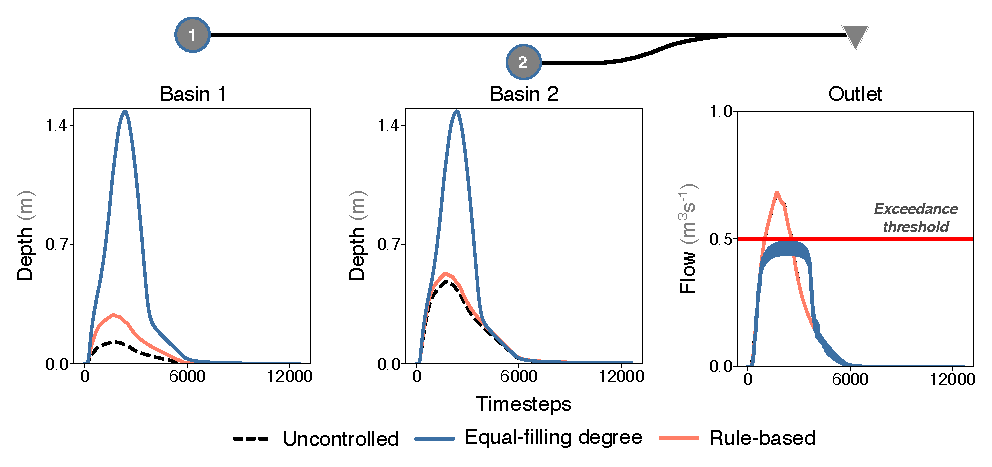
\includegraphics[width=\linewidth]{gfx/Chapter-5/equalfilling.eps}
    \caption{In Scenario \scenario{theta}, the equal-filling degree control strategy is successfully able to maintain the flows at the outlet of the watershed below the desired threshold of $0.5 \unit{m^3s^{-1}}$ by uniformly using the storage in the networks. Static rule-based control and uncontrolled responses of the networks are also presented for comparison. The maximum depth in each of the two basins is $2 \unit{m}$.}
    \label{fig:results}
\end{figure}
%
%
%
\begin{table}[ht]
\small
\caption{Calculated performance metric values from Equation~\ref{eq:perf-sub} for  simulations corresponding to the two implemented control algorithms and the uncontrolled simulation. As can be seen, the equal-filling degree control strategy performs better than the rule-based control strategy, which then outperforms the uncontrolled case.}\label{tab:perfmet}
\begin{tabular}{l c}
\toprule
{\centering \textbf{Control Strategy}} & \textbf{Performance Metric} \\\midrule
Uncontrolled & 1630 \\
Rule-based & 1624 \\
Equal-filling Degree & 0 \\
\bottomrule
\end{tabular}
\end{table}
%
%
%
%
%
%
%
%
%
%
%
%
%
%
%
% -------------------------------------------------------------------------------------------------------------------- %
\section{Discussion}
\label{sec:discussion}
% -------------------------------------------------------------------------------------------------------------------- %
%
%
%
This ability for stormwater systems to be instantly modified is critical as communities prepare for more frequent, uncertain, and destructive weather events due to climate change. More so, \emph{often the most basic control strategies} can have large-scale impacts on the complex, dynamic systems they operate, potentially leading to millions of dollars in savings for the communities they serve. Even though sensor-actuator components may be successfully deployed at individual sites throughout a stormwater network, determining strategies for their coordination across the entire watershed may only add further complexity. As a result, there is a great need --- along with endless opportunities --- to develop and implement novel control strategies for transforming stormwater systems. While the sandboxing efforts of \pystorms serves as an initial effort to foster the development of these strategies, we see specific opportunities to, first, methodically facilitate the development of new simulation frameworks and control algorithms, and subsequently, to then validate and extend their efficacy. We expound on these points here, and discuss next steps to put them into practice.

\

As discussed in Section~\ref{subsec:overviewofthesimulationsandbox}, a critical limitation to progressing smart stormwater control research forward is the inability to systematically develop and analyze smart stormwater simulation workflows and control algorithms. \pystorms can be customized and adapted for a multitude of other uses beyond its initially provided collection of scenarios and stormwater simulator provided. For example, alternative stormwater simulation software be easily integrated into \pystormsNOSPACE.  Furthermore, new scenarios can be assembled from the assortment of components in the scenario collection such that additional research questions can be studied. For instance, for each of the scenarios we provide at the outset, \pystorms specifies only a subset of a scenario's total observable states that are able to be queried throughout the simulation.
However, this initial subset of observable states is never claimed as the optimal; in fact, to the best of our knowledge, there does not yet exist a methodology for identifying an optimal set of observable states. Thus, new scenarios can be made with different subsets of observable states (e.g.\ flows, pollutant concentrations), and new research questions can now be asked about which states may be most critical for informing control actions to be taken.

\

Beyond the coordination and integration of smart stormwater control methods, we view a more expansive opportunity for \pystorms to impel the research community to extend its analysis of \dquote{control.} Specifically, we see a need for improved validation of control methods, and an opportunity for new approaches in defining a control method's success. In the current iteration of \pystorms discussed here, we present a means to assess the performance of a control algorithm via its ability to achieve the pre-defined control objective (e.g. maintain flow below a threshold, avoid flooding). However, there are many other assessment metrics that can define a control algorithm's \dquote{success,} including computational efficiency, applicability across real-world contexts, and the incorporation of social considerations for actual implementation.
\pystorms can serve as a mechanism for assessing the performance of control algorithms across these definitions. For example, by increasing the number of controllable assets available out of the eleven pond outlets presented in Scenario \scenario{gamma}, one can assess the \emph{scalability} of a control algorithm as the state-action space increases. Additionally, control algorithm \emph{generalizability} across storm characteristics can be assessed with the multiple rain events provided in Scenario \scenario{epsilon}. These are just a few illustrations of how \pystorms provides a way to broaden and assess the definition of control efficacy to include factors that are critical for the implementation of smart stormwater approaches in real-world systems.
%
%
%
%
%
%
%
%
%
%
%
%
%
%
%
% -------------------------------------------------------------------------------------------------------------------- %
\section{Conclusions and Next Steps}
\label{sec:conclusion}
% -------------------------------------------------------------------------------------------------------------------- %
%
%
%
\pystorms provides a curated collection of scenarios, coupled with an accessible programming interface, to enable the development and quantitative evaluation of stormwater control algorithms. We have developed \pystorms with the intent to make research into smart stormwater control more accessible to the broader research community. It is our hope that this package will emerge as a community-driven resource that is able to address key knowledge gaps and enable the advancement of smart stormwater systems. To this extent, we see proximate opportunities for the broader research community to collaborate on \pystorms by contributing their own stormwater scenarios and/or control algorithms to the package initiated here. Likewise, we encourage the broader research community to further build upon \pystorms by imparting their own smart stormwater control instances using the \pystorms architecture and integrating their own stormwater control simulation workflows into it.

